\section{Introduction}

\subsection{Motivation}

For a long time the speed of algorithms experienced a constant growth by improved processor hardware. Intel co-founder Gordon E. Moore was one of the first persons to describe this trend in 1965. This description is well known by the name Moore's law which initially stated that the number of transistors on an integrated circuit doubles every year \cite{moore_law}. This trend slowed down and Moore had to change the interval to two years a decade later \cite{moore_law_2003}. The most important consequence however has been realized by one of Moore's co-workers at Intel, David House, who predicted that the performance of processors would double every 18 months \cite{moore_law_2003}. As a result an increase in computing power could be obtained simply by running the same algorithms on newer hardware. As a consequence, hardware dominated the growth of algorithms performance for a long period of time.
\\
Unfortunately, processing hardware technologies hit a limit at the beginning of the third millennium. Physical limits like the size of atoms prevented a further shrink of integrated circuits which would allow an increase in clock speed. Therefore, processor vendors like Intel and AMD started to place multiple CPUs on a single chip which still lead to an increase in computational power but in a different way than in the last 40 years. This change is sometimes referred to as the multicore crisis \cite{multicore_crisis}. The consequence from a software developer's perspective is that traditional algorithms stopped gaining speed by being run on newer hardware. In fact, improving performance is now up to the programmer who is responsible for writing concurrent and parallel software that can make full use of the underlying hardware's capabilities. 
\\
But multicores were not the only major hardware change that had an impact on the way software is developed recently. Graphic cards, which were initially intended to offload and accelerate 2d and 3d graphic operations from the CPU to a separate hardware device, started to gain popularity in non graphical areas of programming. A GPUs intense float processing power and parallel nature by design makes it ideal for uses in several areas of science, business and engineering (General Purpose GPU). When used in the right place, a GPU may compute results several magnitudes faster than the CPU \cite{gpu_history}. However, due to the very different hardware architecture, the graphics card is still not suitable to efficiently solve the same problems as a CPU does.
\\
Todays software engineers working in performance focused domains have a hard time designing their applications and algorithms. With two very different types of processors (CPU and GPU), both excellent in their own ways, and a lot of APIs and frameworks around them (OpenMP, CUDA, OpenCL, DirectCompute, ...), the available hardware and software to access it is more heterogeneous than ever. Thus, profound knowledge of the available technologies, their performance and restrictions as well as the consequences for a development team is essential for choosing the optimal strategy to tackle todays computational needs.

\subsection{Goal}
The goal of this thesis is to provide the reader with a state of the art comparison of modern GPU and CPU performance in solving traditional problems such as sorting arrays and multiplying matrices using various approaches.
The GPU algorithms will be implemented using the Open Computing Language (OpenCL). Therefore the reader is given a short introduction into OpenCL in order to understand the provided code samples and how programming for a GPU works. These OpenCL implementations are benchmarked against algorithms implemented in C/C++ solving the same problem. It is important to note that the GPU and CPU version do not necessarily have to use the same algorithm, they only have to output the same result. This decision was inevitable due to the highly diverse hardware properties of CPU and GPU.
The problems chosen for this comparison are sorting an array, multiplying two large matrices and calculating the parallel prefix sum of an array (explained in corresponding chapter). These algorithms cover several different aspects that play an important role when implementing an algorithm for a GPU such as runtime complexity, memory footprint and memory transfer time vs. computation time. 
\\
Eventually, the results of benchmarking the chosen algorithms should give the reader an idea how much a GPU can accelerate different kinds of algorithms and what a programmer has to pay attention to when developing GPGPU accelerated software. This knowledge is not only valuable during developing, but also useful when choosing the right technology for a given problem. This thesis should aid all software engineers in understanding how GPU computing works and where it should be used.

\subsection{History of GPGPU Computing \cite{gpu_history}} 
Before I start into details about OpenCL and several GPU implementations, I want to provide the reader with some background information about how GPUs have evolved. This may help understanding the design and peculiarities of graphics hardware.
\\



\begin{figure} % from http://http.developer.nvidia.com/CgTutorial/cg_tutorial_chapter01.html
\centering
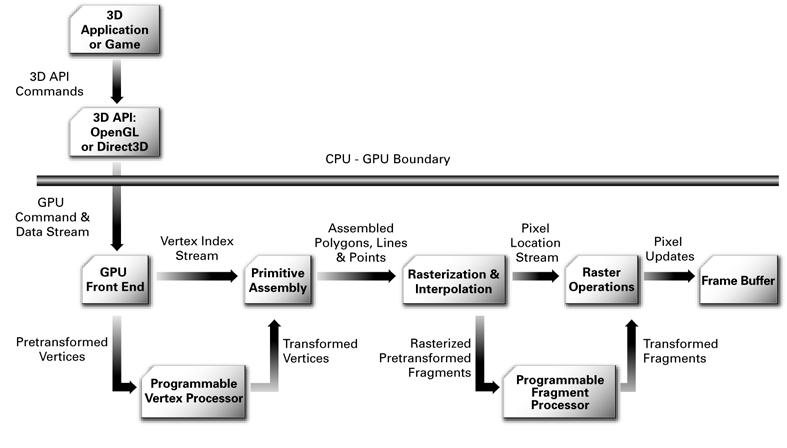
\includegraphics[width=0.7\linewidth]{pipeline2}
\caption{The graphics pipeline with programmable vertex and fragment processor}
\label{fig:pipeline2}
\end{figure}


The development of graphics hardware

shader programming (as first possibility to program for GPUs, focus on graphic calculations, hence the name shader)

Using shaders for GPGPU programming ()

GPGPU Technologies
Cg, CUDA, OpenCL, DirectCompute

\subsection{Chapter overview}


